\title{Midterm - INTD290}
\author{Dr. Jordan Hanson - Whittier College Dept. of Physics and Astronomy}
\date{\today}
\documentclass[10pt]{article}
\usepackage[a4paper, total={18cm, 27cm}]{geometry}
\usepackage{outlines}
\usepackage{hyperref}
\usepackage{graphicx,subfigure}
\begin{document}
\maketitle

\section{How to Submit this Final}

\begin{enumerate}
\item Complete your work on this midterm.
\item Scan it into PDF form using a smartphone app, scanner, or digital picture
\item Alternatively you can type up your answers in a separate file, but it still must be a PDF
\item Submit it using the link on Moodle
\end{enumerate}

\section{Kepler's Laws and The Venus Transit}

\begin{enumerate}
\item \textbf{Kepler's First Law} Given that the \textit{eccentricity} of most planetary orbits is small, we often treat them as a circle.  (a) Why is Pluto different? (b) Suppose we call the radius of the orbit of the Earth around the Sun 1 AU, and 1 AU is $1.5\times 10^8$ km.  What is the orbital radius of Jupiter in km, if we determine it is 5.2 AU? \\ \vspace{3cm}
\item \textbf{Kepler's Third Law} Using Kepler's Second Law, fill in the table in Fig. \ref{fig:plan}.  Compare to the data points in Fig. \ref{fig:plan} (right).
\begin{figure}[hb]
\centering
\begin{tabular}{| c | c | c |}
\hline
Planet & Radius (AU) & Period (years) \\ \hline
Earth & 1.0 & 1.0 \\ \hline
Venus & 0.72 &  \\ \hline
Mars & & 1.88 \\ \hline
Jupiter & 5.2 & \\ \hline
Neptune & & 165 \\ \hline
\end{tabular} \\
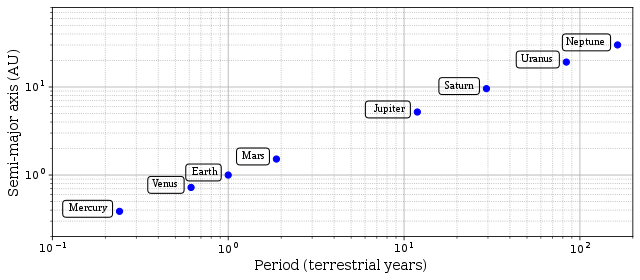
\includegraphics[width=0.5\textwidth]{figures/planets.png}
\caption{\label{fig:plan} Fill in the table using Kepler's Third Law.}
\end{figure}
\item Recently, the European Southern Observatory in the Andes mountains of Chile released results regarding two exoplanets, obtained with the SPHERE instrument on the Very Large Telescope (VLT).  Explain the significance of this result. \\ \vspace{3cm}
\end{enumerate}

\section{Navigation}

\begin{enumerate}
\item Suppose we sail down a river, and use a Cartesian coordinate system to track our progress, in which the positive x-coordinate represents East and the positive y-coordinate represents North.  (a) If we sail from (1.1,1.5) km to (-2.1,1.5) km, what distance did we cover?  (b) In what direction are we heading? \\ \vspace{3cm}
\item Suppose we start at the origin of a coordinate system just like the one in the previous problem. We sail 2 km North, then 2 km East, then 1 km South, then 0.5 km East.  (a) What is our final location?  (b) How far are we away from the origin? \\ \vspace{3cm}
\item Recall that distance is equal to velocity multiplied by time duration.  Suppose that our little boat travels 5 km per hour with the current.  How long is the journey in the previous problem?
\end{enumerate}

\end{document}
